\chapter{Methodology} \label{sec:methodology}


\section{Initial Chunking Strategy for BERT Fine-tuning}

The first preprocessing pipeline was designed to provide a straightforward baseline for fine-tuning. Each conversation was reconstructed from the \textit{dialogue} field into a single string with explicit speaker tags. Tokenization was then applied to the full conversation, with a maximum sequence length of 512 to provide the maximum information context in each chunk, meaning that chunk boundaries could occur in the middle of a message. Conversations exceeding this limit were split into non-overlapping chunks, which could occur at arbitrary positions within the text. Therefore, a single conversation could have multiple chunks, each treated as an independent training example. Finally, dynamic padding was applied at batch time and the tokenized dataset was then passed to the Hugging Face \textit{Trainer} for BERT fine-tuning without additional preprocessing steps such as fixed-length padding or message-boundary control.

\subsection{Train-Test Split}
For the finetuning, a group-level train-test split was applied using \textit{GroupShuffleSplit} from \textit{sklearn}, ensuring that all conversations from a single predator were contained entirely within either the training or test set. This approach prevents data leakage across splits, which could otherwise lead to overoptimistic performance estimates. The split ratio was set to 70\% for training and 30\% for testing. Also, the same ratio of grooming to non-grooming conversations was maintained in both sets to ensure balanced class distributions in the training and train and test data.

The resulting data distribution after chunking is shown in the following table.

\begin{table}[H] 
\label{tab:initial_split} 
\centering
\small
\caption[Initial data distribution after chunking]{\textbf{Initial data distribution after Chunking (max length 512, no message boundary control).}}
\begin{tabular}{lccc}
\hline
Split & Grooming & Non-Grooming PAN12  & \textbf{Total} \\
\hline
Train & 14997 & 30781  & \textbf{45778} \\
Test  & 1330 & 3429   & \textbf{4759} \\
\end{tabular}
\end{table}

\section{BERT fine-tuning as Baseline}

Based on the initial chunking pipeline, BERT was fine-tuned for binary classification. 

The normal baseline followed a classic fine-tuning pipeline for binary classification with \textit{bert-base-uncased}. The training configuration was as follows:

\begin{itemize}
  \item \textbf{Backbone:} \textit{bert-base-uncased} (standard model dropouts)
  \item \textbf{Chunk length:} 512
  \item \textbf{Chunking:} tokenizer-based with \textit{return\_overflowing\_tokens=True}, no overlap, no alignment to message boundaries; dynamic padding in batch
  \item \textbf{Trainer/Optimization:} Hugging Face \textit{Trainer}
  \item \textbf{Epochs:} 3
  \item \textbf{Batch Size:} 8 
  \item \textbf{Learning Rate:} \textit{2e-5}
  \item \textbf{Weight Decay:} 0.01
  \item \textbf{Warmup:} none
  \item \textbf{Gradient Clipping:} not explicitly set
\end{itemize}



\subsection{Evaluation Metrics}
To evaluate the performance of the binary classifier, the most common metrics for a binary classification task were used in \textbf{all the following model evaluations}:

Let $TP$, $FP$, $TN$, and $FN$ denote true positives, false positives, true negatives, and false negatives. 
The metrics are defined as follows:

\begin{align}
\text{Accuracy} &= \frac{TP + TN}{TP + TN + FP + FN}, \\
\text{Precision} &= \frac{TP}{TP + FP}, \\
\text{Recall} &= \frac{TP}{TP + FN}, \\
F_{1} &= 2 \cdot \frac{\text{Precision} \cdot \text{Recall}}{\text{Precision} + \text{Recall}}.
\end{align}

Therefore, Accuracy measures the overall proportion of correctly classified instances, while precision measures the fraction of predicted positive instances that are true positives. 
Recall measures the fraction of actual positive instances that are correctly identified, emphasizing the model's ability to minimize false negatives. 
Finally, the $F_{1}$-score is reported as the harmonic mean of precision and recall, providing a balanced measure that accounts for both. 

Since the dataset is slightly imbalanced, the $F_{1}$-score for the positive class is used as the primary metric, ensuring that both precision and recall are equally considered to make the evaluation robust against class imbalance.

The evaluation was performed every 3000 steps during training, using the test dataset.

\section{Limitations of Initial BERT Fine-tuning Approach}

\textbf{While the initial fine-tuning apporach enabled a fast and effective baseline, it also raised methodological concerns:}
\begin{enumerate}
  \item \textbf{Domain Leakage:} Since all PJ conversations carry label 0 and all PAN12 conversations label 1, the model could rely on dataset-specific artifacts (domain leakage) instead of semantic cues. As a result, the model might learn to distinguish between datasets rather than genuine grooming patterns.
  \item \textbf{Length Leakage:} In addition, PJ conversations are generally longer than the ones from PAN12 (Figure ~\ref{fig:conversation_word_lengths}), making conversation length itself a potential shortcut (length leakage). As a result, the model could exploit systematic length differences rather than learning meaningful grooming-related features.
\end{enumerate}

\textbf{As shown later in the evaluation (Table ~\ref{tab:bert_base}), the initial model indeed achieved very high performance, which motivated the design of a stricter preprocessing pipeline.} Therefore, a second preprocessing script was developed, which introduced fixed-length padding strategies, enforced chunking at message boundaries, and incorporated synthetic non-grooming data in PJ style to reduce both domain and length leakage. The following sections describe this improved pipeline in detail.

\section{Chunking Strategy for BERT to reduce Domain and Length Leakage}

To mitigate leakage effects and evaluate robustness, a stricter preprocessing pipeline was implemented. Instead of splitting conversations at arbitrary positions, chunks were created only at message boundaries, ensuring that single utterances remained intact.

During development, additional options such as random left/right padding and random message shuffling were tested. While these techniques can increase robustness by preventing the model from overfitting to position-specific cues, they were not retained in the final pipeline. There were two reasons for this descision: first, later feature fusion with LIWC required that padding positions remain consistent, otherwise token-level interpretability would be undermined. Second, SHAP was planned as an explainability method, and artificially shuffled or randomly padded inputs would have introduced noise, making it harder to attribute predictions to relevant linguistic or psychometric features.

To further mitigate domain leakage and length leakage, synthetic non-grooming chats in PJ style were added (Section~\ref{sec:synthetic-data}). Models were then trained and tested under two complementary setups: 

\begin{enumerate}
  \item \textbf{Separated Split:} With synthetic data only in the test set, to probe generalization.
  \item \textbf{Mixed Split:} With synthetic data included in both train and test sets, to strengthen robustness.
\end{enumerate}


\subsection{Chunk-Length Distributions (For Train and Test) Across Sequence Lengths}\label{sec:chunk-length-distributions}

To determine the optimal chunk length for a robust BERT baseline the mean, standard deviation, median, minimum, and maximum of tokens per conversation across the different datasets were calculated and are shown in table~\ref{tab:token_stats}. 

\begin{table}[htbp]
\centering
\caption{Token statistics per conversation/file across datasets}
\label{tab:token_stats}
\begin{tabular}{lrrrrrrr}
\toprule
\textbf{Dataset} & \textbf{Files} & \textbf{Mean} & \textbf{Std (pop)} & \textbf{Std (sample)} & \textbf{Median} & \textbf{Min} & \textbf{Max} \\
\midrule
PJ (grooming)                & 6\,175  & 723.83 & 446.54 & 446.58 & 719  & 12  & 1\,850 \\
PAN12                        & 27\,751 & 210.12 & 202.20 & 202.20 & 144  & 1   & 3\,656 \\
Synthetic                    & 621     & 969.47 & 161.24 & 161.37 & 972  & 488 & 1\,435 \\
PAN12 + Synthetic            & 28\,372 & 226.74 & 230.01 & 230.01 & 147  & 1   & 3\,656 \\
ALL (PJ + PAN12 + Synthetic) & 34\,547 & 315.59 & 339.65 & 339.65 & 171  & 1   & 3\,656 \\
\bottomrule
\end{tabular}
\end{table}

The statistics show that PJ conversations are generally much longer (mean: 724 tokens, median: 719 tokens) than PAN12 conversations (mean: 210 tokens, median: 144 tokens). The synthetic conversations are even longer (mean: 969 tokens, median: 972 tokens) and thus closer to the PJ distribution. The combined PAN12 + Synthetic dataset has a mean of 227 tokens and a median of 147 tokens, which is still significantly shorter than PJ. Overall, the complete dataset (PJ + PAN12 + Synthetic) has a mean of 316 tokens and a median of 171 tokens.

To fairly evaluate the base model across these regimes, it was decided to test the baseline training with the following three fixed chunk sizes to evaluate if the chunk size has an impact on performance and model robustness:
\begin{itemize}
  \item \textbf{150 tokens:} closely matches the PAN12 median, minimizing fragmentation for PAN12 while providing a compact, compute-efficient context budget.
  \item \textbf{250 tokens:} offers additional headroom beyond the PAN12 median (covering a larger share of its distribution) and tests whether modestly more context improves performance without a large compute increase.
  \item \textbf{512 tokens:} targets full-length context for longer PJ/Synthetic conversations, reducing truncation and assessing the payoff of richer context windows.
\end{itemize}

Therefore, multiple target sequence lengths (150, 250, and 512) were generated, and padding on these fixed lengths was applied to test the impact of chunk size on performance, preventing the model from relying on systematic length differences between datasets.

Figure~\ref{fig:chunk-dists} shows the resulting chunk length distributions for the three target lengths (150, 250, 512) after applying the improved chunking strategy, to show the impact of different chunk sizes on the dataset. Each subplot displays the distribution of chunk lengths in both training and test sets combined. The orange bars represent grooming chunks collected from PJ, while the blue bars represent non-grooming chunks collected from PAN12. Additionally the green bars show the synthetic non-grooming chunks in PJ style. The Chunk lengths were measured before padding on a fixed size of 512, 250 or 150 chunks was applied.


\begin{figure}[H]
  \centering
  \begin{subfigure}[t]{0.34\textwidth}\centering
    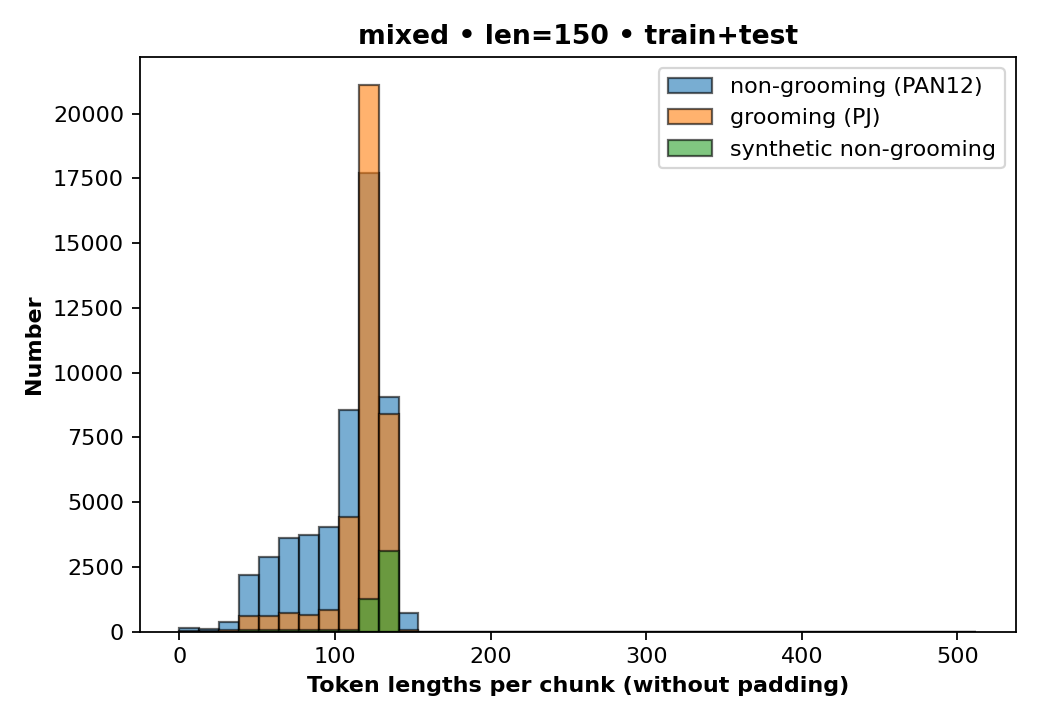
\includegraphics[width=\linewidth]{figures/chunkin_150_dist.png}
    \caption{150 tokens}\label{fig:chunkdist150}
  \end{subfigure}\hspace{-0.5em}% enger rücken
  \begin{subfigure}[t]{0.34\textwidth}\centering
    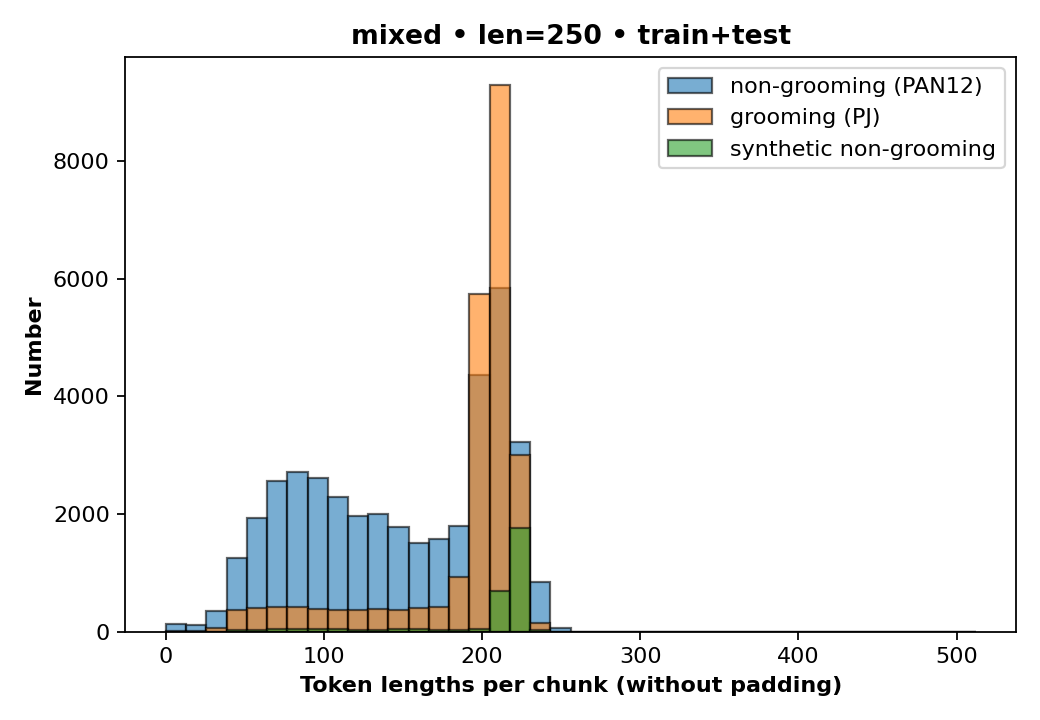
\includegraphics[width=\linewidth]{figures/chunking_250_dist.png}
    \caption{250 tokens}\label{fig:chunkdist250}
  \end{subfigure}\hspace{-0.5em}%
  \begin{subfigure}[t]{0.34\textwidth}\centering
    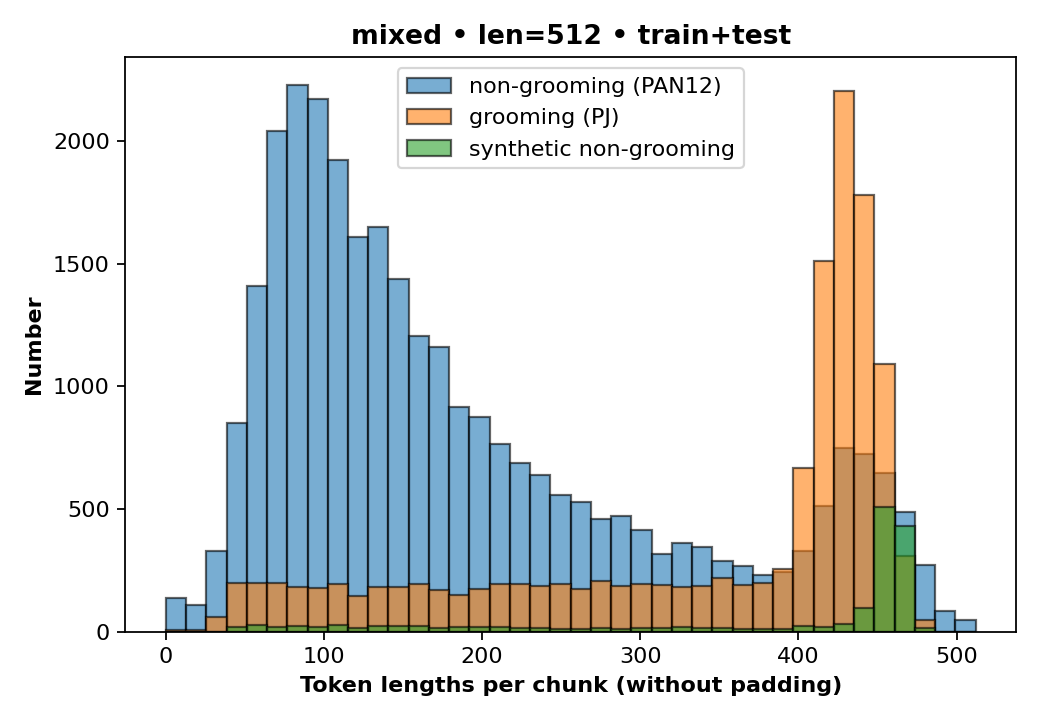
\includegraphics[width=\linewidth]{figures/chunking_512_dist.png}
    \caption{512 tokens}\label{fig:chunkdist512}
  \end{subfigure}
  \caption[Chunk Length Distributions]{Chunk length distributions (train+test) for different sequence lengths (before padding).}
  \label{fig:chunk-dists}
\end{figure}


\subsection{Data Distributions after Chunking}
 The following tables show the resulting data distributions after chunking for the three target lengths (150, 250, 512) and each setup (synthetic data only in test set and synthetic data in test and train set). Each table lists the number of chunks per class in the training and test sets for, together with the total number of chunks. 

 \begin{table}[H]
\centering
\small
\begin{tabular}{lcccc}
\hline
Split & Grooming & Non-Grooming PAN12 & Non-Grooming Synthetic & \textbf{Total} \\
\hline
Separated Train & 27883 & 36954 & 0    & \textbf{64837} \\
Separated Test  &  9625 & 16211 & 4749 & \textbf{30585} \\
\midrule[\heavyrulewidth]
Mixed Train     & 26583 & 37356 & 3254 & \textbf{67193} \\
Mixed Test      & 10925 & 15809 & 1495 & \textbf{28229} \\
\hline
\end{tabular}
\caption[Split for Chunk-Length of 150 Tokens]{\textbf{Split for Chunk-Length of 150 Tokens.}}
\end{table}


 \begin{table}[H]
\centering
\small
\begin{tabular}{lcccc}
\hline
Split & Grooming & Non-Grooming PAN12 & Non-Grooming Synthetic & \textbf{Total} \\
\hline
Separated Train & 17487 & 27057 & 0    & \textbf{44544} \\
Separated Test  &  6003 & 11848 & 2925 & \textbf{20776} \\
\midrule[\heavyrulewidth]
Mixed Train     & 16662 & 27321 & 2008 & \textbf{45991} \\
Mixed Test      &  6828 & 11584 & 917  & \textbf{19329} \\
\hline
\end{tabular}
\caption[Split for Chunk-Length of 250 Tokens]{\textbf{Split for Chunk-Length of 250 Tokens.}}
\end{table}


 \begin{table}[H]
\centering
\small
\begin{tabular}{lcccc}
\hline
Split & Grooming & Non-Grooming PAN12 & Non-Grooming Synthetic & \textbf{Total} \\
\hline
Separated Train & 9699 & 21259 & 0    & \textbf{30958} \\
Separated Test  & 3267 & 9195  & 1583 & \textbf{14045} \\
\midrule[\heavyrulewidth]
Mixed Train     & 9197 & 21352 & 1087 & \textbf{31636} \\
Mixed Test      & 3769 & 9102  & 496  & \textbf{13367} \\
\hline
\end{tabular}
\caption[Split for Chunk-Length of 512 Tokens]{\textbf{Split for Chunk-Length of 512 Tokens.}}
\end{table}



\section{Improved Training Pipeline} \label{sec:improved-training-pipeline}


For training on this improved dataset, the same BERT backbone was used but with a slightly more robust training configuration. Dropout rates in the classification head were increased (0.3), and label smoothing (0.1) was applied to reduce overconfidence. Gradient checkpointing was enabled for memory efficiency. 

\subsection{Improved Training Configuration}

The training configuration for the improved pipeline was the following:

\begin{itemize}
  \item \textbf{Backbone:} \textit{bert-base-uncased} with increased dropouts
  \item \textbf{Sequence length:} Variants \(\in \{150, 250, 512\}\) 
  \item \textbf{Dropout (BERT):} \(\textit{hidden\_dropout\_prob}=0.3\), \(\textit{attention\_probs\_dropout\_prob}=0.3\)
  \item \textbf{Loss function:} Cross-Entropy 
  \item \textbf{Label smoothing:} \(0.1\) 
  \item \textbf{Epochs:} \(3\)
  \item \textbf{Batch size:} \(8\)
  \item \textbf{Learning rate:} \(2\times10^{-5}\)
  \item \textbf{Weight Decay:} \(0.01\)
  \item \textbf{Warmup Ratio:} \(0.06\)
  \item \textbf{Max Grad Norm:} \(1.0\)
  \item \textbf{Gradient Checkpointing:} enabled 
\end{itemize}


\subsection{Evaluation Strategy with Additional Subsets}

The model was trained and tested across all three chunking target lengths (150, 250, 512) under two different setups
\begin{enumerate}
\item \textbf{Synthetic data only in the test set.}
This setup was designed to evaluate whether the model can generalize to PJ-style negatives without having seen them during training.
\item \textbf{Synthetic data in both train and test sets.}
This setup was designed to test whether including synthetic negatives in the training phase improves robustness and reduces reliance on dataset-specific artifacts.
\end{enumerate}

The evaluation was again performed every 3000 steps on the test set, using accuracy, precision, recall, and F1 score as metrics. 

To further test robustness, an evaluation callback ran three subsets after each evaluation step:
\begin{itemize}
\item \textbf{Real-only test set (consisting of only PAN12 + PJ data).}
\item \textbf{Synthetic-only test set.}: Here the model was only evaluated based on the accuracy since precision, recall, and F1 are not defined for a single class.
\end{itemize}

Additionally the confusion matrix was calculated for the complete test set after each evaluation step to analyze the types of errors made by the model. Also, the ROC-Curve and the AUC score were calculated after each evaluation step to analyze the model's performance across different classification thresholds.

The detailed outcomes the training across alle different chunk size and train/test split configurations are shown in the evaluation section (Section~\ref{sec:bert_chunk_size_and_data_setup}).

\section{Choosing the final configuration for Feature Fusion and SHAP Explainability Analysis} 

%%Überarbeitet

Based on the evaluation across different chunk sizes and dataset configurations (Section \ref{sec:bert_chunk_size_and_data_setup}), \textbf{it was decided to continue the feature fusion and explainability analysis with a chunk size of 512 tokens in combination with the mixed split strategy}. Although shorter chunks were hypothesized to reduce length leakage, the results show no significant performance improvement for 150 or 250 tokens. Instead, 512-token chunks consistently achieved the best F1 scores (up to 0.97) while at the same time providing richer conversational context, which is crucial for a clean LIWC analysis. Moreover, the separated split revealed poor generalization, indicating overfitting on training data. By contrast, the mixed split setup led to more robust performance across evaluation subsets, making it the more reliable and realistic configuration for further experiments. Therefore, this final choice balances model accuracy with interpretability and robustness, setting a solid foundation for the following feature fusion experiments and shap analyses.


\section{Choosing the LIWC Feature Set for Feature Fusion and SHAP Explainability Analysis} \label{sec:liwc-feature-selection}

%% überarbeitet


\textbf{The Feature-Fusion and following SHAP explainability analysis was performed with two variants of feature sets in each case: }
\begin{enumerate}
    \item \textbf{All-Features-Fusion}: Use of all 118 LIWC features.
    \item \textbf{Psychometric-Fusion}: Use of a subset of \textbf{49 psychometric LIWC features} coverings all psycholinguistic LIWC features that are highlighted in the literature as relevant for manipulative communication in Grooming Chats (Section \ref{psychometric_liwc_features_in_grooming}). The subset contains the following categories and dimensions:
\end{enumerate}

\paragraph{Psychometric LIWC Subset (49 features).}
\begin{itemize}
  \item \textbf{Drives}: \textit{Drives}, \textit{affiliation}, \textit{achieve}, \textit{power}, \textit{reward}, \textit{risk}, \textit{curiosity}, \textit{allure}
  \item \textbf{Cognition}: \textit{Cognition}, \textit{allnone}, \textit{cogproc}, \textit{insight}, \textit{cause}, \textit{discrep}, \textit{tentat}, \textit{certitude}, \textit{differ}, \textit{memory}
  \item \textbf{Affect \& Emotion}: \textit{Affect}, \textit{tone\_pos}, \textit{tone\_neg}, \textit{emotion}, \textit{emo\_pos}, \textit{emo\_neg}, \textit{emo\_anx}, \textit{emo\_anger}, \textit{emo\_sad}, \textit{swear}
  \item \textbf{Social}: \textit{Social}, \textit{socbehav}, \textit{prosocial}, \textit{polite}, \textit{conflict}, \textit{moral}, \textit{comm}, \textit{socrefs}, \textit{family}, \textit{friend}, \textit{female}, \textit{male}
  \item \textbf{Physical/Biological}: \textit{Physical}, \textit{health}, \textit{illness}, \textit{wellness}, \textit{mental}, \textit{substances}, \textit{sexual}, \textit{food}, \textit{death}
\end{itemize}
\textbf{The idea for this two-staged approach was to evaluate whether a set of only psycholinguistically relevant features could provide similar or better interpretability and performance compared to using the full LIWC-2022 feature set.} 


\section{LIWC Data Extraction}

The LIWC features were extracted using the official LIWC-22 software. The extraction was done once over complete PJ and PAN12 conversations as well as the synthetic non-grooming conversations in PJ style. Furthermore, the LIWC features were also extracted for each chunk in the improved chunked dataset with a chunk size of 512 tokens(Section \ref{sec:methodology}).

Also, the LIWC Features were extracted in two variants: once with all 118 features and once with the psychometric subset of 49 features (Section \ref{sec:liwc-feature-selection}). The extracted LIWC features were then stored in a separate sidecar file.

\section{LIWC Data Analysis}

In order to analyze the effect size of LIWC features prior to fine-tuning, a comprehensive analysis of LIWC features across all conversations was performed.
The LIWC-based analysis was carried out in two steps. First, a global comparison was performed on complete conversations, followed by a chunk-based comparison using 512 chunks, which was tailored to the subsequent feature fusion. Both analyses were performed once for the complete set of LIWC-2022 features and once restricted to the psychometric subset of LIWC features to determine whether psychometric variables alone are sufficient to distinguish grooming conversations from non-grooming conversations.

\subsection{Global LIWC Analysis on Complete Conversations}

For the global analysis, all grooming conversations from the PJ were first aggregated into one conversation per groomer to represent their general language style, while non-grooming conversations from PAN12 were used in their original form. 
For each conversation, the complete set of LIWC-2022 features was calculated.  
To improve interpretability, the features were grouped into macro categories according to the LIWC-2022 manual:

\begin{itemize}
    \item \textbf{Linguistic:} Function, pronoun, ppron, i, we, you, shehe, they, ipron, det, article, numeral, preposition, auxiliary verb, adverb, conjunction, negation, verb, adjective, quantity
    \item \textbf{Punctuation:} Period, comma, question mark, exclamation mark, apostrophe, other
    \item \textbf{Emoji:} Emoji
    \item \textbf{Drives:} Belonging, Achievement, Power
    \item \textbf{Motivation:} Reward, Risk, Curiosity, Enticement
    \item \textbf{Cognition:} Cognition, allnone, cogproc, Insight, Cause, Discrepancy, Attempt, Certainty, Difference, Memory
    \item \textbf{Affect:} Positive tone of voice, negative tone of voice, emotion, positive emotion, negative emotion, fear, anger, sadness, swearing
    \item \textbf{Social:} Social behavior, prosocial, polite, conflict, morality, communication, social references, family, friend, female, male, social
    \item \textbf{Physical:} Health, illness, well-being, mental, substances, sexual, food, death, physical
    \item \textbf{Perception:} Attention, movement, space, visual, auditory, feeling
    \item \textbf{Culture:} Politics, ethnicity, technology
    \item \textbf{States:} Need, desire, acquisition, lack, fulfillment, fatigue
    \item \textbf{Time:} Time, focus on the past, focus on the present, focus on the future
    \item \textbf{Conversation:} Internet slang, agreement, non-fluency, filler words
\end{itemize}

For each conversation, the value of a macro group was defined as the arithmetic mean of all available member characteristics. Subsequently, the macro group means were averaged across all conversations for each class (PJ vs. PAN12). 
The results were visualized as grouped bar charts (PJ vs. PAN12) sorted by the overall mean \(\tfrac{1}{2}(\overline{g}_{\mathrm{PJ}}+\overline{g}_{\mathrm{PAN}})\) .

In addition to macro group aggregation, each individual LIWC feature was statistically analyzed. For each feature \(f\), the mean and standard deviation across all conversations were calculated per class,
\[
\overline{x}_{\mathrm{PJ}},\ s_{\mathrm{PJ}},
\qquad
\overline{x}_{\mathrm{PAN}},\ s_{\mathrm{PAN}},
\]
followed by the mean difference \(\Delta = \overline{x}_{\mathrm{PJ}} - \overline{x}_{\mathrm{PAN}}\) and Cohen's \(d\) \cite{cohen1988},
\[
d = \frac{\Delta}{s_p},
\qquad
s_p = \sqrt{\frac{(n_{\mathrm{PJ}}-1)s_{\mathrm{PJ}}^2+(n_{\mathrm{PAN}}-1)s_{\mathrm{PAN}}^2}{n_{\mathrm{PJ}}+n_{\mathrm{PAN}}-2}}.
\]


The descriptive statistics and effect sizes were compiled into a summary table for all LIWC features which is provided in the appendix (table \ref{tab:liwc22-categories}).

Furthermore, the 30 LIWC-2022 features with the largest absolute effect sizes \(|d|\) were selected to identify the most discriminative variables. 
This procedure was performed twice. Once for the complete set of LIWC features and once restricted to the psychometric LIWC subset to analyze if psychometric features alone capture the major differences between the two classes. 

To further assess the quality and representativeness of the synthetically generated non-grooming data, an additional global LIWC analysis was conducted comparing PJ Grooming and PAN12 Non-Grooming to the synthetic dataset. 
For each comparison, Cohen’s \(d\) was again computed for all LIWC features, and the top 30 features by absolute effect size were visualized as horizontal bar plots. 
This step was intended to identify potential linguistic deviations between the synthetic and real-world data and to evaluate whether the synthetic data exhibits similar psycholinguistic patterns as PAN12.

The results of the global LIWC analysis are presented in the evaluation section (Section~\ref{sec:global_liwc_analysis}).

\subsection{Chunk-based LIWC Analysis with 512 Tokens}

To examine patterns within conversations, a chunk-based analysis was performed with a fixed chunk size of 512 tokens (identical to the size later used for model training). For each chunk, a LIWC-2022 feature vector was calculated and the average values per class were determined across all chunks. also based on the data level , which
For each feature, the range
\[
\mathrm{range}(f) = \max_{s}\overline{f}_{s} - \min_{s}\overline{f}_ {s}
\]
was determined for each feature across all sources (\(s \in \{\mathrm{PJ}, \mathrm{PAN12}, \mathrm{SYN}\}\)), and the \(K=15\) features with the largest ranges were selected for visualization.
Two heatmaps were created: one limited to these 15 most important distinguishing features and one containing all available features (in alphabetical order).The rows represent PJ Grooming, Synthetic Non-Grooming, and PAN12 Non-Grooming, while the columns represent the LIWC features.
This process was repeated once for all LIWC features and once for the psychometric features to determine whether psychometric variables alone exhibit comparable distinction at the chunk level.

The visualization and evaluation of the chunk-based LIWC analysis is presented in section~\ref{sec:chunk_based_liwc_analysis}.

\section{Feature Fusion Strategy}

%%Überarbeiter

To extend the BERT baseline with the additional input of LIWC features, the LIWC features were first extracted for all chunks from the dataset with 512 tokens and stored as numerical vectors in a separate sidecar file.  For this purpose, the sidecar contained a key consisting of \textit{conv\_id} and \textit{chunk\_index} for each chunk, as well as the corresponding chunk-specific LIWC features. 
When loading the dataset, these sidecar files were assigned to the respective chunks based on the \textit{conv\_id} and the \textit{chunk\_index} (for dialogues consisting of several chunks), so that the training and test data sets then contained an additional column for \textit{liwc} in addition to \textit{input\_ids}, \textit{attention\_mask}, and \textit{labels}. \newline

To integrate the LIWC features into the BERT architecture, \textbf{a late fusion approach} was implemented using cross-attention and a gating mechanism. This method allowed the model to select information from LIWC into the contextualized token representations learned by BERT. 

\subsection{Model Architecture}

The proposed feature fusion model extends \textit{bert-base-uncased} (12 transformer layers, hidden size \(d_h=768\), 12 attention heads) with a late-fusion mechanism that integrates psycholinguistic LIWC features into the transformer encoder in the upper encoder layers at layer 6 and 12. The design was used to keep the original BERT architecture and its pre-trained weights intact while allowing the model to leverage additional psycholinguistic information from LIWC. This keeps the tokenization and main contextual processing of the text unchanged, while the LIWC information is only introduced after language modeling, which holds comparability with the BERT baseline and allows a later downstream explainability using SHAP. The overall process can be summarized as followed:

\begin{itemize}
    \item \textbf{Input and Feature Projection:}
    \begin{itemize}
        \item For each text chunk, a LIWC feature vector \(x \in \mathbb{R}^{d_{liwc}}\) is extracted 
        (\(d_{liwc}=118\) for all features or \(d_{liwc}=49\) for the psychometric subset).
        \item \(x\) is normalized using \textit{LayerNorm} and mapped through a linear projection with \textit{GELU} activation to a compact fusion dimension \(z \in \mathbb{R}^{d_p}\) (\textit{proj\_dim}, e.g., 128/768).
        \item From \(z\), a single \emph{LIWC token} \(t \in \mathbb{R}^{d_h}\) is generated via a linear layer. 
        This token summarizes the psychometric information for the entire chunk.
    \end{itemize}

    
    \item \textbf{Fusion via Cross-Attention:}
    \begin{itemize}
        \item Text hidden states \(H \in \mathbb{R}^{T \times d_h}\) from intermediate layers serve as \textbf{queries}.
        \item The LIWC token \(t\) is used as \textbf{key/value} in a multi-head cross-attention mechanism (\textit{n\_heads}=4, mask-aware).
        \item This enables each token to attend to the psycholinguistic context selectively.
    \end{itemize}
    
    \item \textbf{Gating and Residual Update:}
    \begin{itemize}
        \item A channel-wise gate \(g \in \mathbb{R}^{d_h}\) (\textit{gate\_type}=\textit{channel}) is computed from the \textit{[CLS]} representation and \(z\).
        \item The final representation is updated via
        \[
        H' = H + g \odot \mathrm{Attn}(H, t)
        \]
        followed by a 10\% dropout.
        \item A post-fusion \textit{LayerNorm} is applied to stabilize training and normalize the residual update.

    \end{itemize}
    
    \item \textbf{Integration in Encoder:}
    \begin{itemize}
        \item The fusion block is applied in the upper encoder layers (layers 6 and 12; \textit{fusion\_at\_layers} with \textit{depth}=1).
        \item After the final fusion layer, the \textit{[CLS]} vector is pooled as in the baseline model and passed to a linear classification head.
        \item  The pooled \textit{[CLS]} representations are combined either by averaging (\textit{mean}). The resulting fused representation is then passed to the linear classifier.

    \end{itemize}
\end{itemize}
    
    

The overall feature-fusion architecture is illustrated in the following figure~\ref{fig:liwc-bert-fusion}.

\begin{figure}[H]
    \centering
    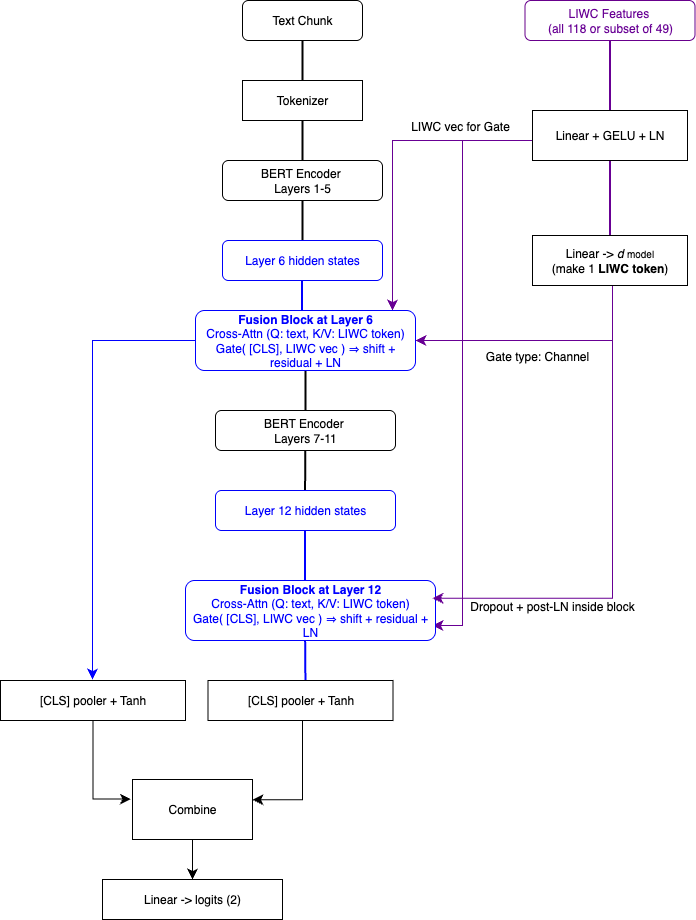
\includegraphics[width=0.7\textwidth]{new_fusion.png}
    \caption[Feature Fusion Architecture]{Late fusion of LIWC with BERT: LIWC features (either all 118 or the 49 psychometric subset) are projected, transformed into a single \emph{LIWC token}, and fused with hidden states from layers 6 and 12 via cross-attention plus a gating mechanism (Multimodal Shifting). The resulting fusion blocks are applied in parallel to the BERT encoder and do not feed back into subsequent layers. The [CLS] representations from both fusion points are pooled, combined, and classified. The \textcolor{blue!70!black}{blue blocks} highlight where fusion takes place, while the \textcolor{violet!70!black}{purple line} represents the LIWC stream (projection and token).}
\label{fig:liwc-bert-fusion}

\end{figure}

\subsection{Training Pipeline and Evaluation}

The training and evaluation of the feature fusion model followed a similar pipeline as the improved BERT-Baseline (Section~\ref{sec:improved-training-pipeline}). With the following hyperparameters:

\begin{itemize}
\item \textbf{Number of Epochs:} \(3\) 
\item \textbf{Saving Checkpoint at Epoch:}\(1\) 
\item \textbf{Evaluation Steps:} \(3000\)
\item \textbf{Learning Rate:} \(2\times10^{-5}\)
\item \textbf{Weight Decay:} \(0.01\)
\item \textbf{Warmup Ratio:} \(0.06\)
\item \textbf{Max Grad Norm:} \(1.0\)
\item \textbf{Batch Size:} \(8\)
\item \textbf{Loss Function:} Cross-Entropy with Label Smoothing of \(0.1\)
\item \textbf{Dropout inside Fusion} \(0.1\)
\item \textbf{Number of Heads in Cross-Attention:} \(4\)
\item \textbf{Fusion Depth:} \(1\)
\end{itemize}

The Evaluation was performed with the same metrics as in the BERT-Baseline (accuracy, precision, recall, F1) and on the dataset with chunks consisting of 512 tokens and synthetic data in both train and test set. The evaluation was done every 3000 steps of training and the model was stored after each epoch.




\section{Explainability Analysis based on Feature Fusion Model}

The following Analysis was done based on the Feature Fusion Model with a Chunk size of 512 tokens and Synthetic Data in both Train and Test set after \textbf{three epochs of training}. This decision was made to ensure that the model had sufficient exposure to the data and to capture more complex patterns in the feature interactions.

To analyze the model's decision-making process, SHAP was used to show insights into how both token-level text features and LIWC psychometric features contributed to the model's predictions. The following sections describe the two complementary explainability analyses that were conducted.


\subsection{SHAP analysis of LIWC features} \label{sec:shap_analysis_of_liwc_features}

To understand which psycholinguistic features are relevant for the classification decision, a SHAP analysis of the LIWC features was performed. Both the complete LIWC feature set with 118 dimensions and a psychometric subset with 49 selected categories were considered. The fixed-length LIWC vector calculated for each chunk served as input for the analysis. 

\subsubsection{Reducing Computational Costs with KernelSHAP}
The explanations were generated using KernelSHAP, whereby the text input of the model was capped to a fixed sequence length and kept constant for all explanations. To keep the computational costs of the SHAP analysis manageable, a fixed configuration was used for both the complete LIWC feature set (118 dimensions) and the reduced psychometric subset (49 dimensions). Specifically, \texttt{64} random samples from the test set were selected for explanation. For the background distribution, \texttt{32} LIWC vectors were chosen and reduced to at most 20 representative centroids using k-means clustering. Each instance was then perturbed \texttt{256} times in order to approximate the marginal feature contributions. 

The model was executed in mini-batches of \textit{4} explanations, with a maximum of \textit{16} perturbations processed in parallel. In addition, the text input was capped to a constant sequence length of \texttt{64} tokens, and inference was carried out in mixed precision with disabled gradients. These measures reduced GPU memory consumption and made it feasible to perform KernelSHAP for both feature sets without exceeding hardware limits.

\subsubsection{Determing Feature Importance and Direction of Effect}

For each instance in the test dataset, the prediction for the positive grooming class was explained. SHAP determines how much the model prediction changes when a single LIWC feature is neutralized. A high SHAP value indicates that this feature contributed significantly to the decision. In this way, the \textbf{mean absolute} SHAP value (\emph{mean $|$SHAP$|$}) was calculated for each LIWC feature, describing the global importance of the feature. To make the results easier to interpret, these values were then converted into percentages of the total significance:

\[
\text{FeatureImportance}_{i} = \frac{\text{mean}\,|SHAP|_{i}}{\sum_{j=1}^{F} \text{mean}\,|SHAP|_{j}} \times 100 \%
\]

where \(F\) is the number of LIWC features. This shows the percentage of the total model decision that can be explained by a single feature (Figure \ref{fig:global_feature_importance_combined}).

In addition, the \textbf{mean signed} SHAP value was determined to indicate the direction of the effect.
Therefore \textbf{a positive SHAP value means the feature pushes the prediction toward the positive class (grooming), while a negative SHAP value means it pushes toward the negative class (non-grooming). Thus, higher projected values indicate more grooming-like language, lower values indicate more non-grooming-like language.}
The results were summarized in several steps and can be found in section \ref{sec:ablation_studies_shap}.



\subsection{Confidence Analysis based on Label Flip and Confidence Shift}

In order to further investigate the impact of LIWC features on model decisions, model confidence and class assignment were calculated once with the regular LIWC feature vectors (\emph{LIWC on}) and once with LIWC vectors set to zero (\emph{LIWC off}). This allowed the influence of the additional LIWC features on model confidence and class assignment to be analyzed.

For both conditions, the class probability was determined by applying the softmax function to the logits. The highest probability \(p_{\max}\) represents the model confidence for the predicted class:
\[
p_{\max}^{(\text{on})} = \max_k p_k^{(\text{LIWC on})}, \qquad
p_{\max}^{(\text{off})} = \max_k p_k^{(\text{LIWC off})}.
\]

The difference between these two values defines the so-called \textbf{confidence shift}:
\[
\Delta p_{\max} = p_{\max}^{(\text{on})} - p_{\max}^{(\text{off})}.
\]
A positive value indicates that the LIWC features increased the certainty of the model decision, while a negative value describes a decrease in confidence.

In addition, it was analyzed whether the predicted class of an input changed as a result of LIWC fusion (for example, model decision = grooming before and model decision = non-grooming after). If such a change occurs, it is referred to as a \textbf{label flip}:
\[
\text{flip} = \mathbb{1}\!\left[\,\hat{y}^{(\text{on})} \neq \hat{y}^{(\text{off})}\,\right], 
\qquad
\hat{y} = \arg\max_k p_k.
\]
The number and rate of label flips show the extent to which the LIWC features lead to a changed classification decision.

For quantitative analysis, the following metrics were calculated:
\begin{itemize}
    \item $\Delta \mu$, $\Delta \tilde{x}$, $\Delta \sigma$: Mean, median, and standard deviation of \(\Delta p_{\max}\).
    \item $\Delta p_{10}$, $\Delta p_{90}$: 10th and 90th percentiles of the distribution of \(\Delta p_{\max}\).
    \item $n_{\text{class 0}}$, $n_{\text{class 1}}$: Frequency distribution of the predicted classes with LIWC.
    \item $n_{\text{flips}}$, flip rate: Number and relative frequency of prediction changes.
\end{itemize}


The results are presented in Section ~\ref{sec:confidence_and_label_flip_analysis}.

\section{LIWC Analysis of Misclassifications}

To identify potential patterns in the misclassifications made by the feature fusion model, a LIWC analysis of false positives and false negatives was conducted. It was tested whether misclassified samples resemble the opposite correct class in LIWC space, i.e., whether false negatives are closer to true negatives and false positives are closer to true positives according to their LIWC Feature values. Furthermore, it was analyzed which LIWC features differ significantly between misclassified and correctly classified samples. This analysis was again conducted with both the full LIWC feature set and the psychometric subset. The same fusion model, tokenizer, and LIWC sidecar vectors as in the previous sections were used to generate predictions and per-sample LIWC vectors. The analysis was performed on the complete test set.

\subsection{Descriptive per-group statistics}
For each LIWC feature and each confusion group \(g \in \{\mathrm{TN},\mathrm{TP},\mathrm{FP},\mathrm{FN}\}\), the following descriptive statistics were computed over the per-sample values:
\[
\text{count},\;\text{mean},\;\text{std},\;\text{median},\;\text{q1 (25th)},\;\text{q3 (75th)},\;\text{min},\;\text{max}.
\]
These summaries describe central tendency and spread within groups and are used as context for the inferential tests below. The complete summary statistics for all LIWC features are provided in the appendix (table \ref{tab:liwc22-misclassification-stats}).

\subsection{Per-feature group comparisons}
Per-feature comparisons were run for four group pairs: FP vs.\ TN, FN vs.\ TP, TN vs.\ FN, and TP vs.\ FP. For each LIWC feature \(f\), let \(x\) denote values in the first named group and \(y\) in the second. The following statistics were computed:

\begin{itemize}
\item \textbf{Mean difference} \(\Delta\mu = \bar{x} - \bar{y}\).
\item \textbf{Again, Cohen's \(d\)  was used to quantify effect size}
\item \textbf{Significance tests.} The Mann–Whitney \(U\) test (two-sided) was used to assess the significance of differences in distributions of FP/TN and FN/TP.
\item \textbf{Multiple testing control.} The Benjamini–Hochberg procedure was applied across features to obtain FDR-adjusted \(q\)-values. For plotting, a significance score \(-\log_{10}(q)\) was used.
\end{itemize}


\subsection{Proximity hypothesis tests in LIWC feature space}
To test whether misclassifications resemble the opposite correct group in LIWC space, distances were computed in standardized feature space (z-scored per LIWC dimension). Let \(\mathbf{c}_{\mathrm{TN}}\) and \(\mathbf{c}_{\mathrm{TP}}\) be the centroids of TN and TP, respectively. For each FN sample with standardized vector \(\mathbf{z}\), Euclidean distances
\(d_{\mathrm{TN}} = \|\mathbf{z}-\mathbf{c}_{\mathrm{TN}}\|_2\) and
\(d_{\mathrm{TP}} = \|\mathbf{z}-\mathbf{c}_{\mathrm{TP}}\|_2\) were computed and the following one-sided hypotheses were tested:
\[
H_{1}^{\mathrm{FN}}:\; \Pr\!\big[d_{\mathrm{TN}} < d_{\mathrm{TP}}\big] > 0.5
\quad\text{and}\quad
H_{1}^{\mathrm{FP}}:\; \Pr\!\big[d_{\mathrm{TP}} < d_{\mathrm{TN}}\big] > 0.5.
\]
For each hypothesis, the analysis reports:

\begin{itemize}
  \item \textbf{Proportion of samples} closer to the hypothesized centroid:
  \[\hat{p} = \frac{1}{n}\sum_{i=1}^{n} \mathbb{1}[d_{\text{closer}} < d_{\text{farther}}].\]
  \item \textbf{One-sided binomial test} against \(0.5\) to assess whether the observed proportion \(\hat{p}\) is significantly greater than chance.
  \item \textbf{Paired one-sided tests} on the distance differences \(d_{\mathrm{TN}} - d_{\mathrm{TP}}\) for FN and \(d_{\mathrm{TP}} - d_{\mathrm{TN}}\) for FP. Both the Wilcoxon signed-rank test and the one-sample \(t\)-test were used to assess whether the mean/median difference is significantly greater than zero.
\end{itemize}

The results of the LIWC analysis of misclassifications are presented in section \ref{sec:misclassification_analysis}.

\subsection{SHAP-Based Proximity Analysis of Top-20 Misclassifications}


For a deeper analysis of misclassifications, an evaluation was performed based on the \textbf{top 20 LIWC features}, which were identified in Section~\ref{sec:shap_analysis_of_liwc_features} as the most relevant using global SHAP values (\emph{mean\_abs}) and explain the majority of model decisions. This allows examining whether misclassifications can be explained by their proximity to the opposite correct class along these LIWC dimensions. Also, focusing on the 20 most important features reduces noise from less informative variables and enables a more targeted analysis of group differences.

\paragraph{Top-K selection and SHAP direction.}
All LIWC-2022 features were globally ranked by their \emph{mean\_abs} SHAP values, and the top 20 were selected. In addition, the SHAP sign (\emph{mean\_signed}) was used for each feature to define the “TP-like” versus “TN-like” direction.

\paragraph{Z-scaling and SHAP-oriented projection.}
To ensure comparability, feature columns were z-scaled. The values were then multiplied \emph{per sample} by the SHAP sign (\(+1\) or \(-1\)). On this aligned axis, values \emph{to the right of \(x=0\)} correspond to greater TP similarity, while values \emph{to the left of \(x=0\)} indicate greater TN similarity. The dashed vertical line at \(x=0\) in the plots marks this separation threshold.

\paragraph{Group statistics and confidence intervals.}
For each group (\(\{\mathrm{TP}, \mathrm{TN}, \mathrm{FP}, \mathrm{FN}\}\)) and each top-K feature, group means \(\bar{x}\), standard deviations \(s\), and standard errors
\[
SE \;=\; \frac{s}{\sqrt{n}}
\]
with \(n\) as the group size were calculated. For the misclassification groups (FP and FN), a 95\% confidence interval was then computed:
\[
\mathrm{CI}_{95} \;=\; \bar{x} \pm 1.96 \cdot SE.
\]
The position of this CI relative to \(x=0\) was classified as:
\begin{itemize}
  \item \emph{TP-side}: \(\mathrm{CI}_{95}\) lies completely to the right of 0 (clearly TP-like),
  \item \emph{TN-side}: \(\mathrm{CI}_{95}\) lies completely to the left of 0 (clearly TN-like),
  \item \emph{crosses-0}: \(\mathrm{CI}_{95}\) includes 0 (ambiguous),
  \item \emph{unknown}: no CI could be computed (e.g., missing SE).
\end{itemize}

\paragraph{Proximity rate (distance logic).}
Additionally, for each feature it was assessed which correct class the misclassifications were closer to. This was determined using the distances between the misclassification mean \(\bar{x}_{\mathrm{MC}}\) and the TP or TN means:
\[
d_{\mathrm{TP}} = \lvert \bar{x}_{\mathrm{MC}} - \bar{x}_{\mathrm{TP}} \rvert, \qquad
d_{\mathrm{TN}} = \lvert \bar{x}_{\mathrm{MC}} - \bar{x}_{\mathrm{TN}} \rvert.
\]
For \textbf{FP}, features with \(d_{\mathrm{TP}} < d_{\mathrm{TN}}\) (closer to TP) were counted. For \textbf{FN}, features with \(d_{\mathrm{TN}} < d_{\mathrm{TP}}\) (closer to TN) were counted. The proportion across all top-K features yields the \emph{proximity rate} (e.g., 0.75 = 75\% of features support the expected proximity).

\paragraph{Summary measures.}
The following aggregated values were derived:
\begin{itemize}
  \item \textbf{Proximity rate}: proportion of features supporting the expected proximity (FP\(\rightarrow\)TP or FN\(\rightarrow\)TN),
  \item \textbf{CI TP-side (n)}: number of features with 95\% CI fully to the right of 0,
  \item \textbf{CI TN-side (n)}: number of features with 95\% CI fully to the left of 0,
  \item \textbf{CI crosses 0 (n)}: number of features with 95\% CI intersecting 0 (ambiguous).
\end{itemize}

The results of this analysis, including visualization and summary tables, are presented in Section~\ref{sec:shap_missclassification_analysis}.


